\documentclass{article}
\usepackage{graphicx}
\usepackage{float}

\begin{document}

\title{CS181 Spring 2016 Practical 4: Reinforcement Learning | Team EXT3}
\author{Robert J. Johnson | Dinesh Malav | Matthew McKenna}


\maketitle

\begin{abstract}
Swingy Monkey is a very basic game written in Python. Our project focused on using this game as a simplified context to develop and gain exposure to reinforcement learning algorithms. By implementing a variation of Q-Learning, our study showed that after 200 epochs, our score was able to reach 1,016, a vast improvement over random movements from the monkey.
\end{abstract}
\section{Technical Approach}
Initially, we conducted cursory research on different approaches that were available utilizing reinforcement learning. Based on the YouTube video included in the practical specification, we decided our main focus would be an implementation of  a particular reinforcement learning algorithm, Q-Learning. We then coded up a solution in Python to develop a policy for the monkey to navigate the course. In basic terms, Q-Learning is an unsupervised learning algorithm that essentially stores value information regarding a particular approach to an outcome-based event in a matrix and uses this matrix to make further decisions in later epochs. We attempted to implement the process described at:
$$http://mnemstudio.org/path-finding-q-learning-tutorial.htm$$\\
Two major problems arose initially that constrained our implementation. The first major issue was how to interpret the incoming stream of objects in the jungle. In Swingy Monkey, we are faced with what is essentially a continuous input of data, and thus, we decided early on that the best way to for both ourselves and the algorithm to interpret the position space was to discretize the playing field into 'bins. The second issue was the algorithm's ability to infer how the gravity changes during each epoch of the game. Since the pattern is random, we had to quickly find a way to deduce what the rate was in order to determine our policy for navigating the trees.\\\\
Our implementation of the algorithm begins by getting the current state of the monkey and the forest. The ultimate goal for the algorithm is to learn which actions have the greatest "reward" and use this information combined with the current input to maximize utility and make informed decisions regarding the next action to take. Our reward information is stored in matrix $R$ and our information on learned rewards is stored in a similar matrix $Q$.\\\\
Two functions ended up doing the bulk of the work for the solution. The first was $action\_callback$.\\\\
The results of $action\_callback$ were eventually passed over to $reward\_callback$.
\section{Results}
Our monkey was trained to reach an average score of 48.7 after 200 epochs, with a maximum score of 1,016.  As expected, the average score increased dramatically as the number of epochs increased and the algorithm learned how to control the monkey based on the Q matrix. Around epoch 175, we saw a score above a thousand, and a few other scores above 600 after about 150 epochs:  \\

%\graphcispath{ {c:\ml\kaggle\comp4\Practical4\} }
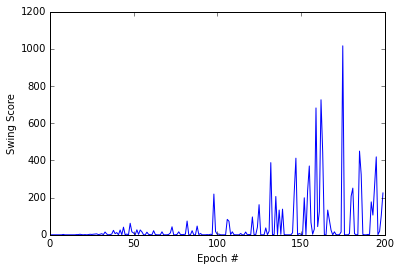
\includegraphics[scale=.7]{score_epoch.png}

We also tried changing the values of the  hyper-parameters to see how they would affect the swing score.  After trying various values of epsilon and bin size, we found that a bin size of 50 and an epsilon value of .001 gave the highest average swing score:  

\begin{center}
\begin{tabular}{ |c|c|c| } 
\hline
 {Epsilon} &  {Bin size}  &  {Avg. Swing Score} \\ 
 \hline
  .01 & 10 & 0.63 \\
  .01 & 50 & 7.1\\  
 .001 & 50 & 48.7 \\
 .001 & 100 & 4.0 \\
 .0001 & 50 & 25.5 \\  

\hline
\end{tabular}
\end{center}

The bin size had a big effect on the swing score.  Changing the bin size even slightly would produce results that were significantly worse compared to using a bin size of 50.  When using a bin size of 10, the maximum score we saw was 9, compared to 1,016 with a bin size of 50.  

\section{Discussion}
The implementation discussed here is not perfect, and there are other reinforcement learning approaches that we could have explored. Q-Learning was selected due to its ease of implementation and potential to effectively implement a policy for the monkey's traversal. Research in reinforcement learning is rapidly changing and evolving, so there will likely newer and more novel solutions developed for similar discrete problems such as this.\\\\
All code for this project can be found at: $$https://github.com/HarvardCS181Practical2016$$.





\end{document}